\chapter{DEFINITIONS}
% !TEX root = hazy1.tex

\section{Overview}

This section defines many of the quantities used by \Cloudy.  I try to
follow standard notation, such as that used by \citet{Mihalas1978} or AGN3.
Other parts of this document goes into many of these quantities in greater detail.

This document has the following typographic conventions;
\cdFilename{filename},
\cdTerm{variable},
\cdCommand{command},
\cdTerm{jargon},
\experimental\ experimental commands,
\cdVariable{variable name},
and \cdRoutine{routine name}.

\section{Radiation fields}

Figure \ref{fig:radiation_fields} shows several of the
radiation fields computed in the calculation.
%2.1
\begin{figure}
\centering
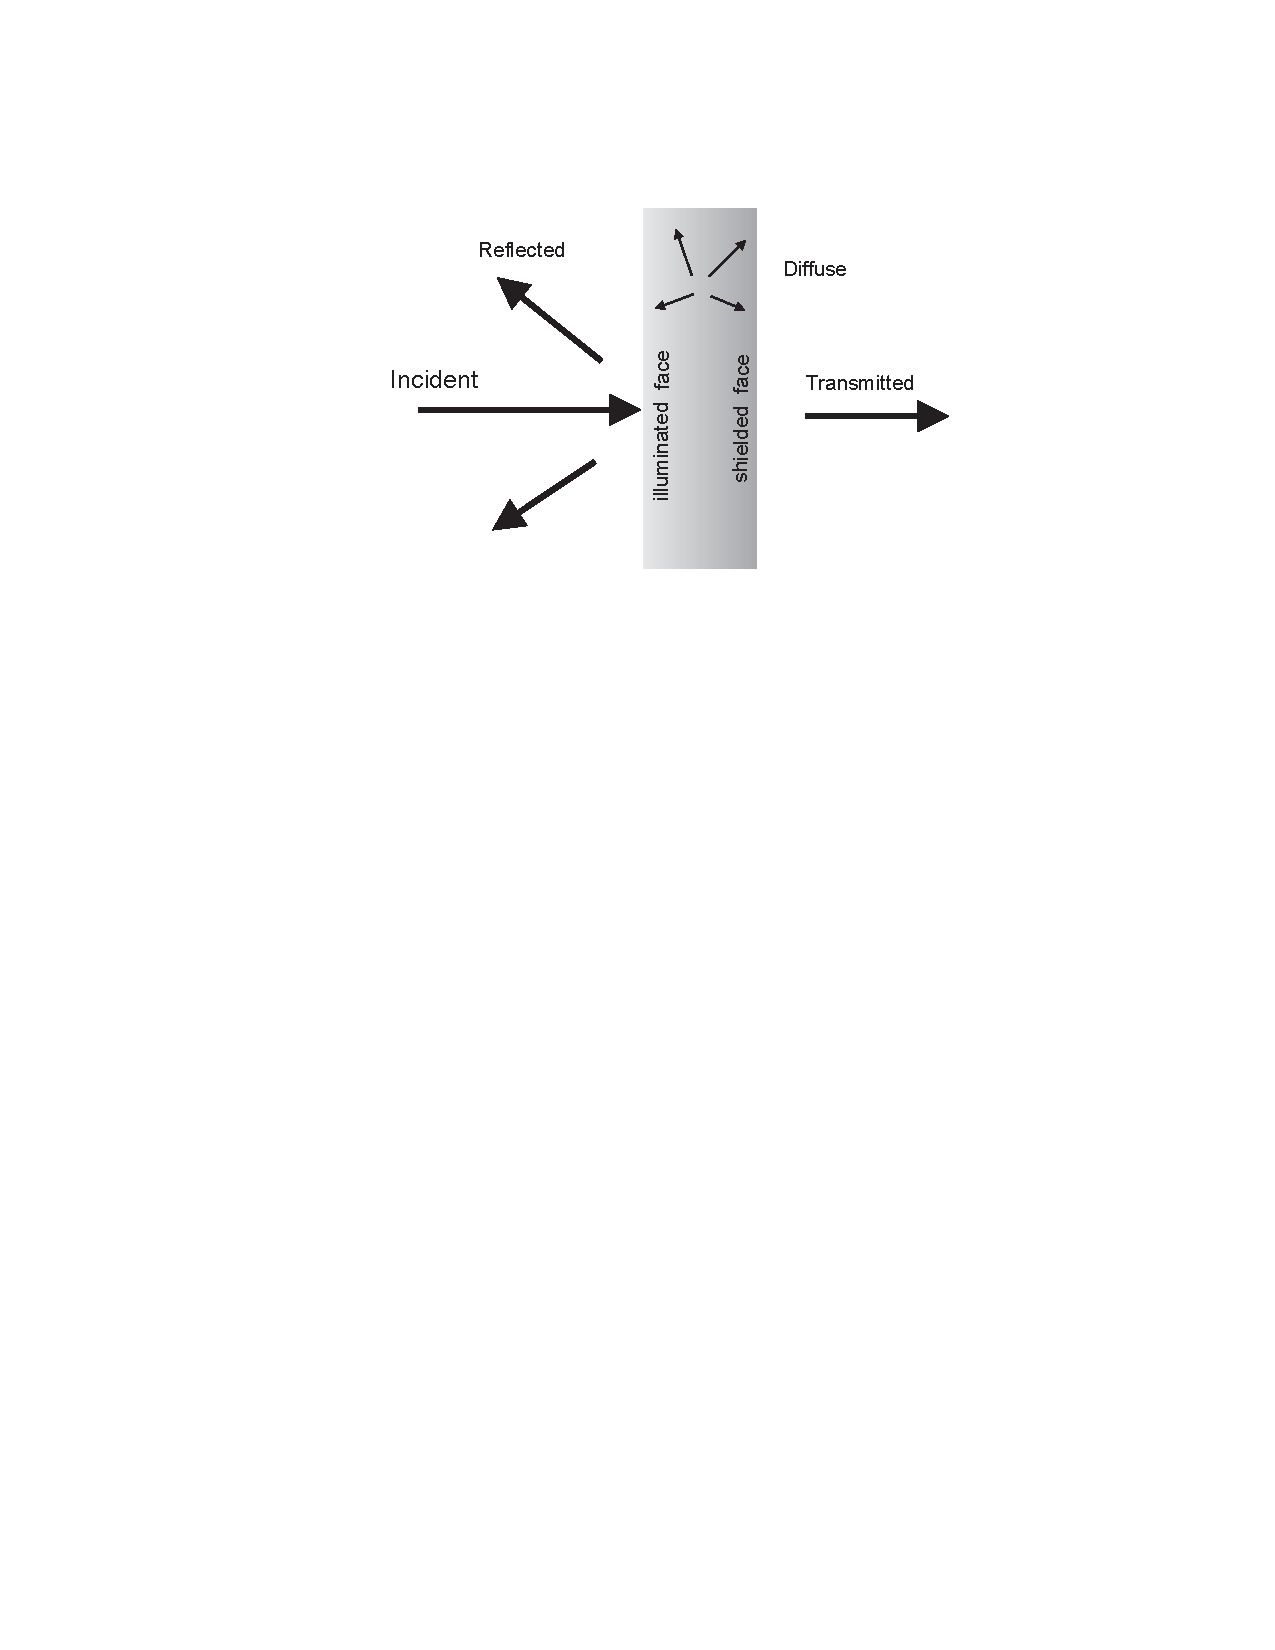
\includegraphics{radiation_fields}
\caption[Contributors to total radiation field]{Several of the radiation fields that
enter in the calculations.}
\label{fig:radiation_fields}
\end{figure}

\subsection{Incident radiation field}

The \cdTerm{incident radiation field} is the external radiation field emitted by the central
object that strikes the \cdTerm{illuminated face} of the cloud.
It is specified in
the commands that set up the calculation.
Often the incident field
is the only energy source for the cloud.
As the incident radiation field is
transmitted through the cloud it is diminished by extinction.

\subsection{Diffuse radiation field }

The \cdTerm{diffuse radiation field} (often referred to as the
diffuse fields) is the radiation field emitted by gas and grains within
the nebula.  Examples include the Lyman, Balmer, or two-photon continua
emitted by hydrogen.  These fields are very nearly isotropic and can be
significant sources of ionizing radiation under some circumstances.

The main difference between the calculation of a stellar atmosphere and
a photoionized cloud is in the treatment of the diffuse fields.
The gas
albedo, which gives the relative probability of a photon being scattered
versus being absorbed, is generally small in a nebula.
As a result, the
diffuse fields must be far weaker than the attenuated incident continuum
since the second is usually the cloud's only real energy source.
The total radiation field is usually dominated by the attenuated
incident radiation field.
By contrast
in a stellar atmosphere the nearly isotropic diffuse field usually dominates
the local intensity.
As a result the diffuse fields can be treated by lower
order approximations in a photoionized cloud than in a stellar atmosphere.

\subsection{Transmitted radiation field}

The \cdTerm{transmitted radiation field} is the net
emission emergent from the shielded
face of the cloud.
It includes both the \cdTerm{attenuated incident} and
the \cdTerm{diffuse} radiation fields.

\subsection{Reflected radiation field}

The \cdTerm{reflected radiation field} is the emission
from the illuminated
face of the cloud back into the direction towards
(i.e., within $2\pi$~sr of)
the source of the external field.
The reflected field is the result
of both backscattered incident radiation and diffuse emission emitted from
the cloud towards the source of ionizing radiation.
This component is only
computed for an \cdTerm{open geometry} (defined below).

Figure \ref{fig:incident_reflected} shows a plot of the incident and
reflected radiation fields for the Compton reflector in an AGN.
This is a large column-density cloud, $N(\mathrm{H}) = 10^{23.75}$
cm$^{-2}$, illuminated by a $f_v\propto v^{-1}$ power law.
The incident radiation field is shown as a
dashed line and the reflected radiation field, obtained from the \cdCommand{save continuum} command),
is the solid line.
The Compton reflector's peak at X-ray
energies is clearly shown.

\begin{figure}
\centering
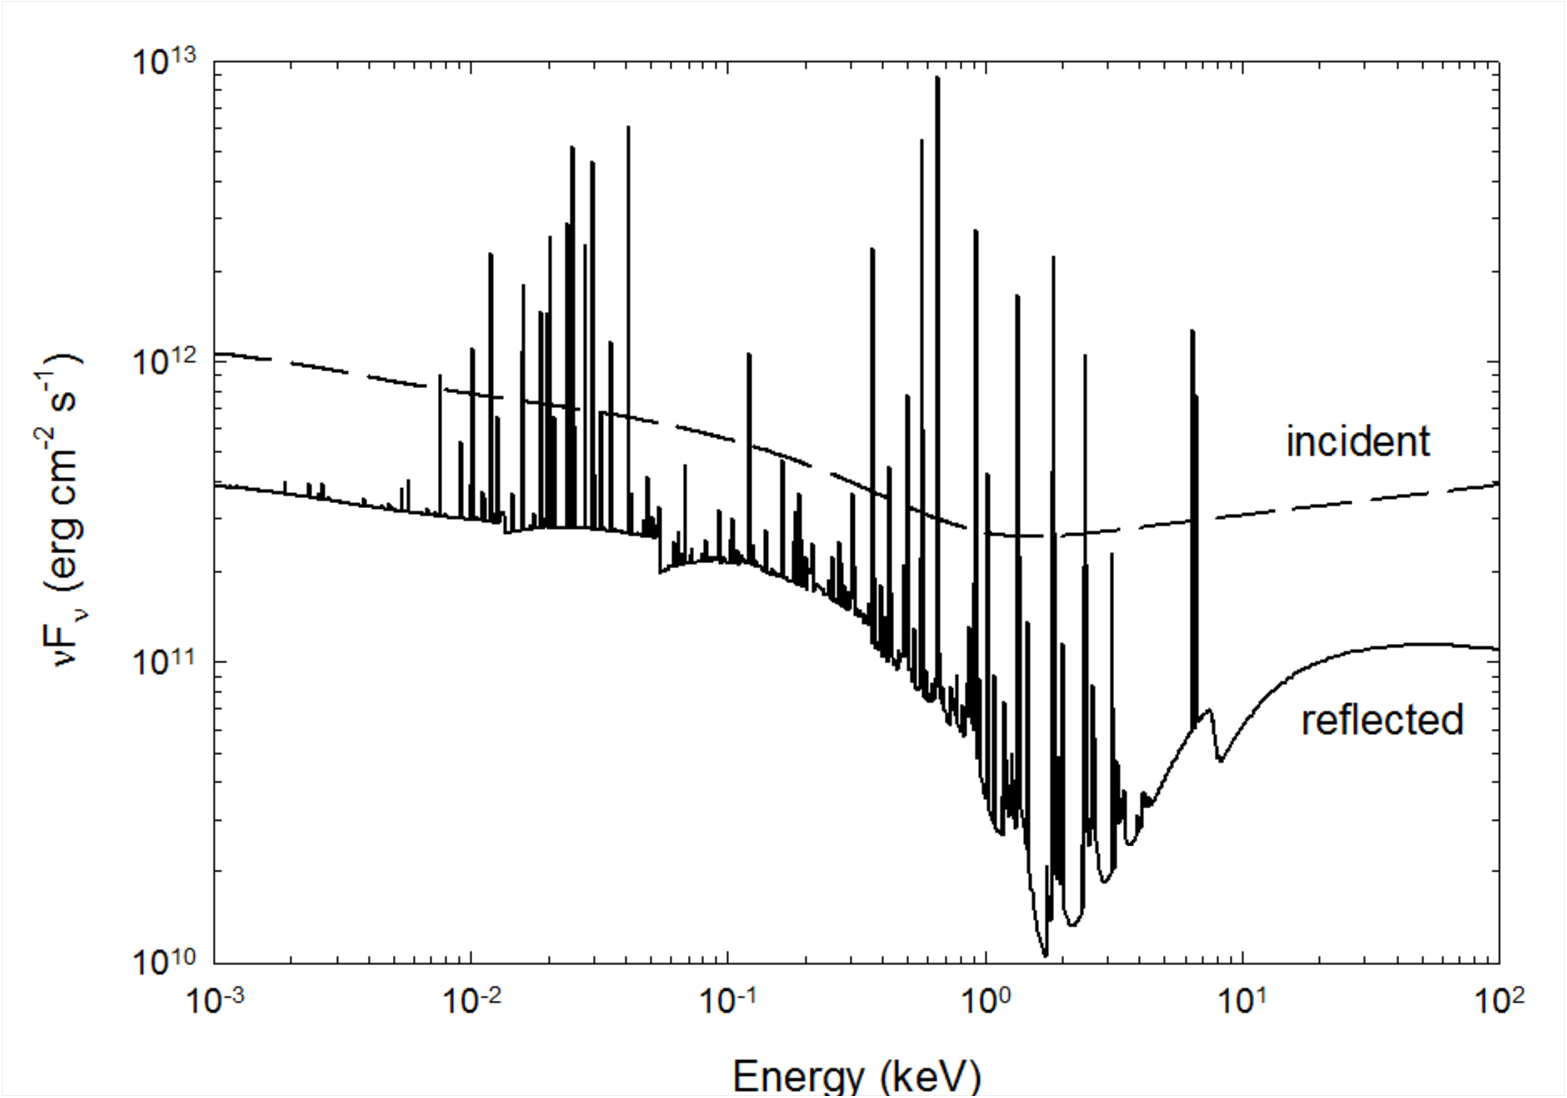
\includegraphics[scale=0.7]{incident_reflected}
\caption[Incident and reflected radiation field]{This incident (dashed) and reflected (solid)
radiation fields,
as computed by agn\_blr\_albedo.in in the test suite.}
\label{fig:incident_reflected}
\end{figure}

\section{Geometry}

In the simplest case the geometry is spherical, or plane
parallel if the inner radius is much larger than the thickness of the
cloud.
The summary at the end of the calculation will
say whether the geometry was plane parallel  (the ratio of the thickness
to the inner radius, $\Delta r/r_o < 0.1$), a thick shell ($\Delta r/r_o <
3$), or spherical
($\Delta r/r_o \ge 3$).

Complex geometries are done by using Cloudy to compute volume elements
within a much larger cloud.
An example is the Cloudy\_3D code,
available from 
\href{http://sites.google.com/site/cloudy3d/}{sites.google.com/site/cloudy3d}
and described in \citet{MorissetCloudy3D06}
and \citet{MorissetStasinskaCloudy3D08}.
Cloudy\_3D was used to compute
the images shown on the cover and in Figure~\ref{fig:Cloudy3D}.
The RAINY3D code is another example 
\citep{MoraesDiazRAINY09}.

\begin{figure}
\centering
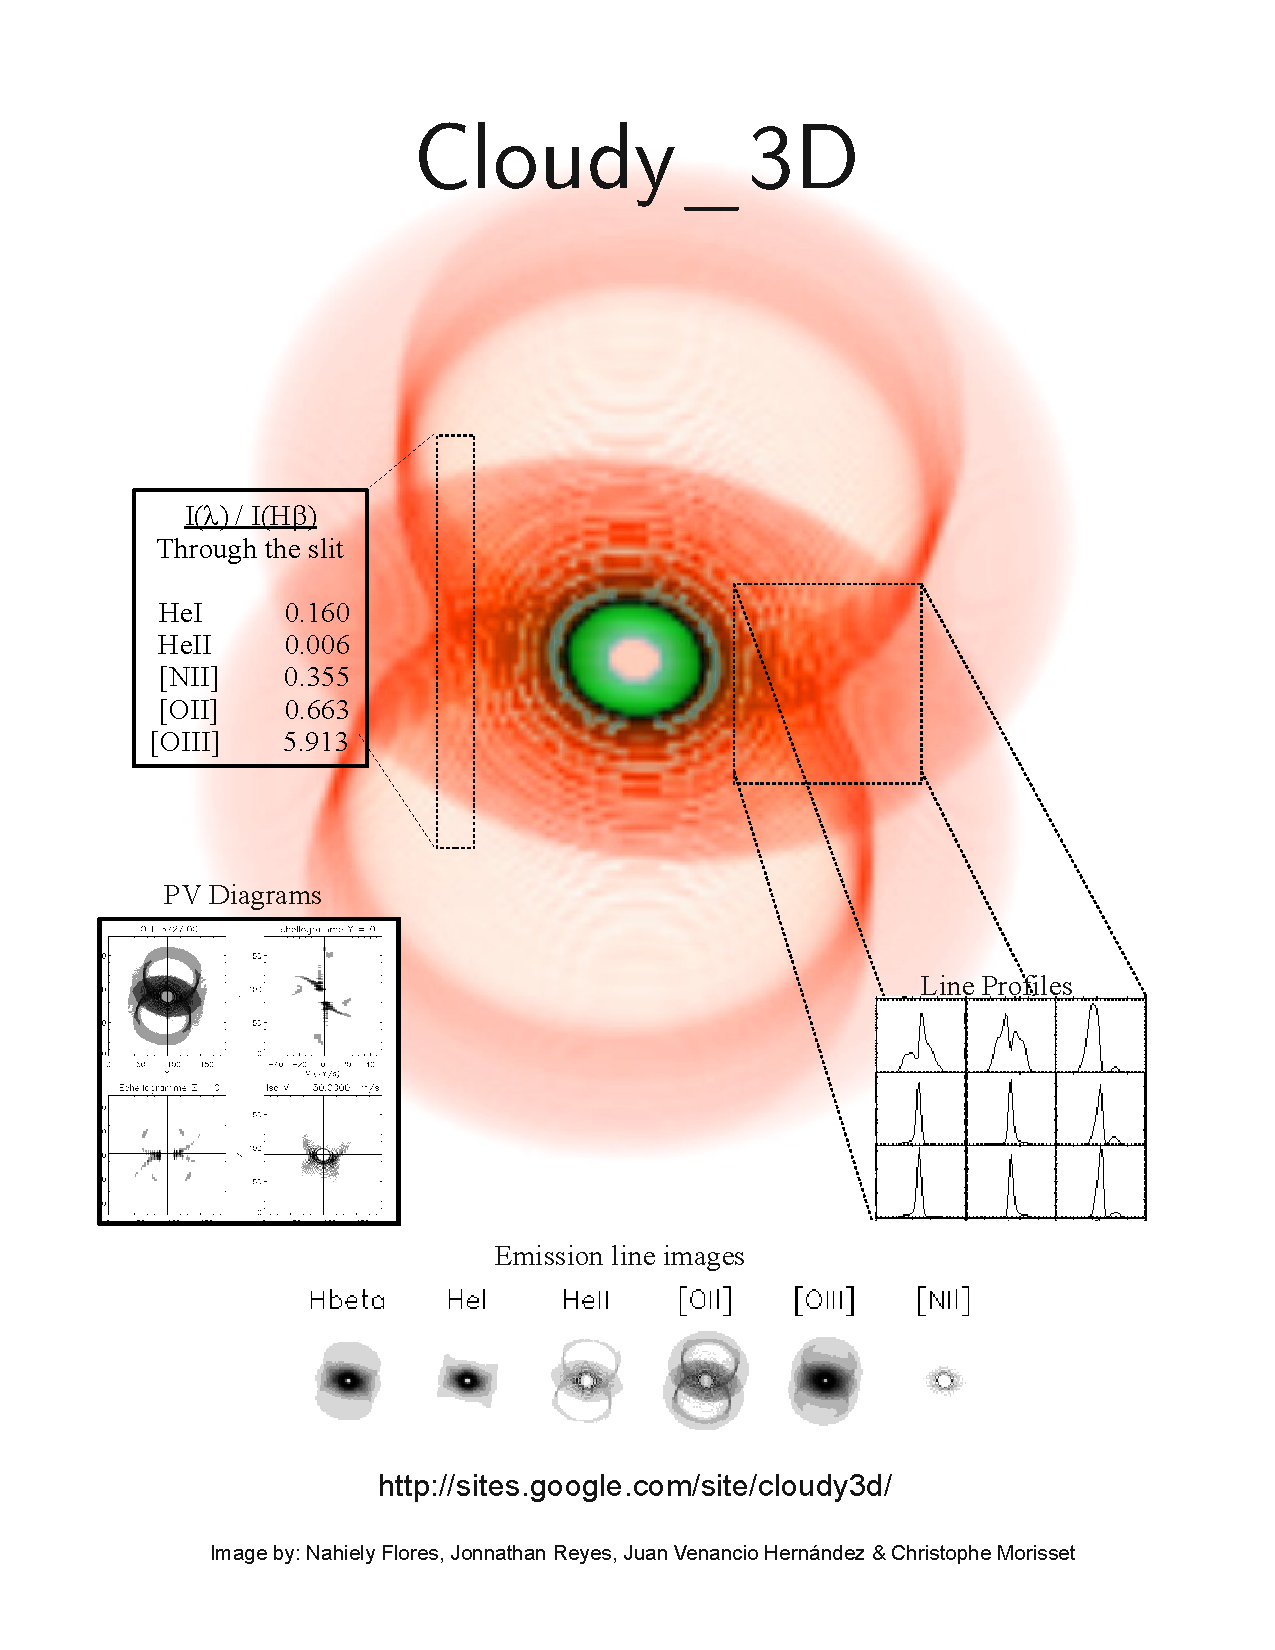
\includegraphics[width=\columnwidth]{posterhazy02}
\caption[Cloudy\_3D simulation of a planetary nebula]
{A 3-color image of a Hourglass-type nebula, 
obtained by running Cloudy 3D.
Colors are [\nii ] (orange) and [\oiii ] (green) emission. 
Emission line profiles are shown for [\nii ] lines. 
Intensities through any given slit can be obtained. 
Position-velocity diagrams are obtained as well as
channel maps, for any line. 
Emission line surface brightness maps are
also available for any line computed by \Cloudy. 
Statistical tools to
analyze emission line properties are also provided.}
\label{fig:Cloudy3D}
\end{figure}

\subsection{Illuminated and shielded faces of the cloud}

The side of the cloud facing the source of the external radiation field
is the \cdTerm{illuminated face} of the cloud.
The opposite side, in shadow, is the \cdTerm{shielded face} of the cloud.  
The illuminated face is generally
hotter and more highly ionized than the shielded face.
In nearly all cases the calculation starts at the illuminated face and stops at the shielded face.

\subsection{Depth and radius}

Figure \ref{fig:GeometryOpenClosed} shows two possible geometries
and some terms used to describe them.
The \cdTerm{radius} is the distance from the center of symmetry,
usually the center of the central object, to a given point.
The \cdTerm{depth} is the distance
between the illuminated face of the cloud and a point within the cloud.
The \cdTerm{inner radius} is referred to as $r_o$,
the depth is $\Delta r$, and the \cdTerm{current radius} is $r$.
The depth or radius for a zone is the distance to the center of the zone.

\begin{figure}
\centering
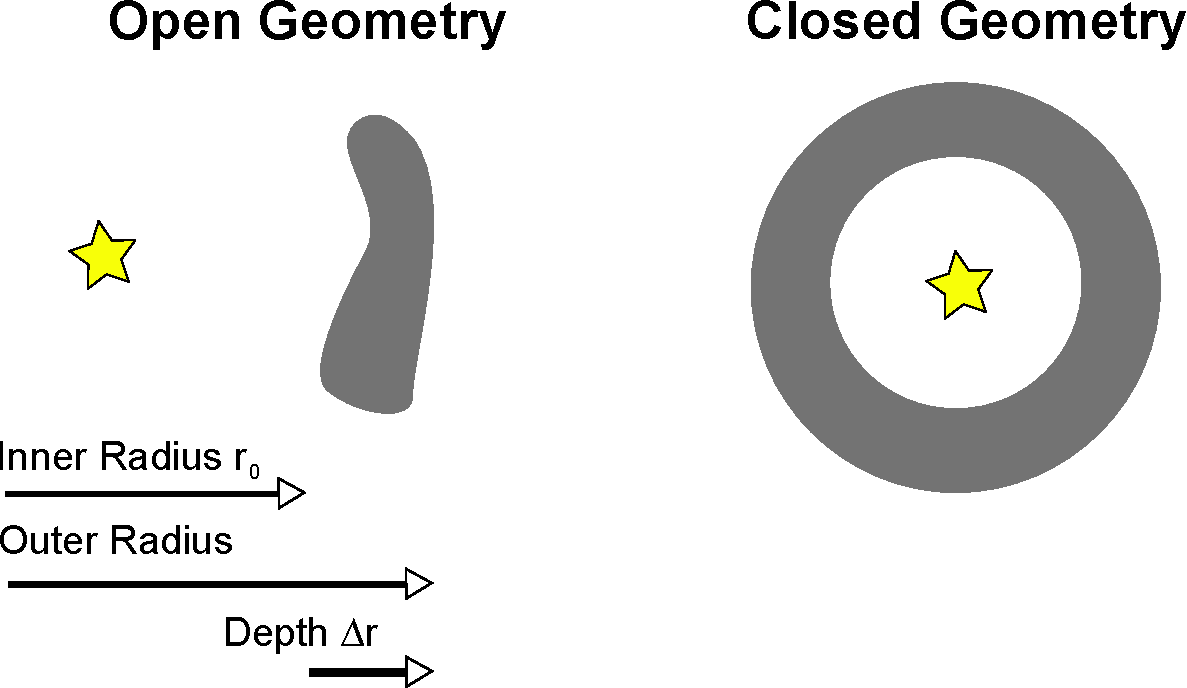
\includegraphics[scale=0.5]{GeometryOpenClosed}
\caption[Open and closed geometries]
{This figure shows the two limiting cases that can be assumed.
The star is the source of ionizing radiation and the shaded area represents
the cloud. An open geometry is the default, and a closed geometry will be
computed if the \cdCommand{sphere} command is entered.}
\label{fig:GeometryOpenClosed}
\end{figure}

\subsection{Covering factor}

The \cdTerm{covering factor} is the fraction of $4\pi$~sr
covered by gas, as viewed
from the central source of radiation.
It is normally written as $\Omega/4\pi$ (AGN3 Section 5.9),
has the limits $0\le\Omega /4\pi\le 1$,
and is the fraction of the
radiation field emitted by the central object
that actually strikes nebular gas.
\cdTerm{Line luminosities} give the total energy emitted by
a shell covering
$\Omega$~sr while \cdTerm{line intensities} give
the energy emitted per unit area of cloud.
Line luminosities scale nearly linearly with increasing covering factor
while line intensities are only weakly dependent on it.

\subsection{Open vs. closed geometry}
\label{sec:GeometryOpenClosed}

Two limiting cases, referred to as \cdTerm{open} and \cdTerm{closed}, can be identified
for the geometry and its influence upon the calculations.
Figure \ref{fig:GeometryOpenClosed} shows
examples of both.
The covering factor determines which is the best
approximation.
The choice mainly affects the transfer of the diffuse fields
and has only second-order effects on predicted quantities.

\begin{description}
\item[Open geometry.]
An \cdTerm{open} geometry is one in which the covering factor
of the gas is small. All radiation that escapes from the illuminated face
of the cloud, towards the source of continuous radiation, then escapes from
the system without further interaction with gas. This is thought to be
the case in, for example, the broad-line region of active nuclei or a blister
H~II region.  In this case L$\beta$ and higher hydrogen Lyman lines and ionizing
radiation produced by recombinations can escape from the nebula.  This
geometry is the default and will be assumed if the \cdCommand{sphere} command is not specified.

\item[Closed geometry.]
Emission-line gas covers ${\sim}4\pi$ sr as seen by the central
object in a \cdTerm{closed} geometry.
The central object is small relative to
the nebula then all diffuse fields which escape from the illuminated face
of the cloud in the direction towards the central object will go on to strike
the far side of the nebula.
This geometry is implicitly assumed in most
calculations of planetary nebulae and \hii\ regions.
This geometry will be
assumed if the \cdCommand{sphere} command is entered.

\item[Static vs. expanding.]
The sphere command has two optional arguments,
\cdCommand{static} and \cdCommand{expanding}.  This determines how emission-line photons which cross
the central hole and strike the far side of the shell interact with the
gas.  The \cdCommand{static} option says to assume that the shell is stationary so that
all lines interact across the nebula.  In this case hydrogen Lyman line
interaction should ensure that Case~B is reached (AGN3 Section 4.2).  If
the nebula is expanding then the continuum photons that cross the central
hole will interact with gas on the far side but the expansion velocity of
the shell ensures that diffuse line photons do not.  In this case the
\cdCommand{expanding} option should be set.  This second case is the default
when \cdCommand{sphere}
is specified with no options.

\emph{Don't panic!}  These geometrical considerations (open vs closed, static
vs expanding) make only second-order differences in the predicted
emission-line spectrum, generally at the ${\approx}10$\% level, largely because of
the different treatments of the radiative transfer of the diffuse fields.
If you are concerned about which geometry to use, try both, and compare
the results.  The differences are usually small.
\end{description}

\subsection{Filling factor}

The \cdTerm{filling factor} $f(r)$ accounts for clumping
of emission-line gas.
When a filling factor is set the hydrogen density is the density within
regions containing gas while surrounding regions are assumed to be a vacuum.
The specific effects of a filling factor are described by \citet{Osterbrock1959} and in AGN3 section 5.9.

\subsection{Hydrogen density}

The \cdTerm{hydrogen density} $n(\mathrm{H})$ is the
total hydrogen density given by
\begin{equation}
n(\mathrm{H}) = n(\mathrm{H}^0) + n(\mathrm{H}^+) + 2n(\mathrm{H}_2)+\sum_{other}
n(\mathrm{H}_{other})\ [\mathrm{cm}^{-3}]
\end{equation}
where $n(\mathrm{H}_{other})$ represents H in all other hydrogen-bearing molecules.

\subsection{Column densities}

The \cdTerm{hydrogen column density} $N$(H) is given by
\begin{equation}
N(\mathrm{H})= \int n (\mathrm{H})\, f(r) \, dr \ [\mathrm{cm}^{-2}]
\end{equation}
where $f(r)$ is the filling factor.   I try to consistently use lower case
$n$ for a volume density (cm$^{-3}$) and an upper case $N$ for
a column density (cm$^{-2}$).

\subsection{Matter-bounded and radiation-bounded geometries}

Two limiting cases for the hydrogen-ionization structure of a cloud exist.

\begin{description}
\item[Matter-bounded geometry.]
The cloud is said to be matter bounded if
the outer limit to the \hplus\ region is marked by the
outer edge of the cloud.
In this case the cloud is ionized throughout
and is optically thin to the
incident radiation field.
In a matter-bounded cloud the intensity or luminosity
of an optically thin recombination line is set by
the product of volume and density
(called the emission measure $n^2V$, AGN3, Section 8.1) and is
not directly related to the luminosity of the ionizing continuum.

\item[Radiation-bounded geometry.]
The cloud is said to be radiation bounded
if the outer limit to the \hplus\ region is defined by
a hydrogen ionization
front so both warm ionized and cold neutral regions exist.
The \hplus\ region
is optically thick to the hydrogen-ionizing radiation
and has absorbed nearly all of it.
In this case the intensity or luminosity of a recombination
line is set by the luminosity of the ionizing continuum with
relatively little dependence on cloud properties.
\end{description}

\section{Intensity \& luminosity cases }
\label{sec:IntensityLuminosityCases}

The external radiation field is usually specified with
two different commands.
One specifies the shape of the incident radiation field.
A second command will set the brightness of the light.
\Cloudy\ must be able to deduce the flux of photons
[cm$^{-2}$ s$^{-1}$]
striking the illuminated face of the cloud.
There are two ways to specify the brightness of the external radiation field.

\subsection{Luminosity case}

If the brightness of the external radiation field is specified as a ``luminosity'',
the light radiated by the central object into $4\pi$~sr, then it is also
necessary to specify an inner or starting radius so that the flux of
photons can be derived.

The emission lines will be predicted as luminosities.
A covering factor will linearly change the luminosity of the entire spectrum
but will have only second order effects on relative intensities.

\subsection{Intensity case}

The external radiation field can be specified as an ``intensity'',
the energy
incident upon a unit area of cloud, with units
something like photons cm$^{-2}$~s$^{-1}$.
It is not necessary to specify a starting radius in the intensity case
although it is possible to do so.
Line intensities (energy emitted per
unit area of cloud, related to $4\pi J$)), are predicted in this case.

If the ``intensity'' of the external radiation field is set then a starting radius does not
need to be specified.
If the starting radius is not specified then an inner
radius of 10$^{30}$ cm is assumed.  A plane-parallel geometry usually results.
The predicted emission-line spectrum is then given in intensity units.
A starting radius may be specified and, if it is, then the resulting geometry
may be spherical, plane parallel, or a thick shell, depending on the ratio
of the outer to inner radii.  Both absolute and relative intensities of
lines have only second-order dependencies on the covering factor.

The word ``intensity'' appears in quotes since it is
not the $I$ or $J$ defined in radiative transfer texts, but rather the photon
or energy equivalent of $4\pi J$.

\subsection{The units of the predicted emission lines}

The units of the predicted emission-line spectrum are determined by the
units of the incident radiation field.
If the incident field is specified as a
luminosity then the spectrum will be given as the luminosity radiated by
a shell covering  $\Omega$~sr of the central object ($L_{line}, \mathrm{erg\,
s}^{-1}$).  Here $\Omega$ is the
angular coverage of the nebula so that $\Omega/4\pi$ (with a default value of unity)
is the covering factor (AGN3, Section 5.9).  If the
continuum is specified as an intensity then the spectrum will be the energy
radiated by a unit area of cloud into $4\pi$~sr $(4\pi J_{line}$, erg
cm$^{-2}$~s$^{-1}$).

\section{``Species'', how we specify atoms, ions, and molecules, and their spectra}
\label{sec:SpeciesDefine}

\subsection{Overview}
\Cloudy\ simulates gas ranging from fully ionized to molecular.
Nomenclature varies considerably between chemical, atomic, and plasma physics.
We adopted a nomenclature that tries to find a middle ground between
these different fields.

We refer to a particular atom, ion, or molecule as a ``species''.
A species is a baryon.  Examples are CO, \htwo, H$^+$, and Fe$^{22+}$.
Species are treated using a common approach, as much as possible.
Our naming convention melds a bit of each of these fields
because a single set of rules must apply to all species.

The species are taken from a number of databases and a large
number of commands control how they are used.
These commands are described in the Section beginning on page 
\pageref{sec:ControllingAtomicModels} below.
The commands controling output options for the species are
described in the Section starting on page
\pageref{sec:SaveSpecies} below.

A spectrum is a collection of photons.  Examples that might appear in the literature
are H~I or C~IV.  
It is not convenient to use these labels in computer input/output.
We adopted the following rules.

\subsection{How we specify species and spectra}

Some rules for how these are specified:

\begin{itemize}

 \item
 Labels are case sensitive, to distinguish between the
 molecule CO and the atom Co.
 
 \item
 At present we do not use \verb|_| to indicate subscripts, or \verb|^|
 to indicate  charge.

 \item
 Molecules are written pretty much as they appear in texts.
 \htwo, CO, and H$^-$ would be written as ``H2'', ``CO'', and ``H-''.

 \item 
 Atoms are the element symbol by itself.
 Examples are ``H'' or ``He''
and \emph{not} the atomic physics notation
 H$^0$ or He$^0$.
 
 \item 
 Ions are given by ``+'' followed by the net charge.
 Examples are ``He+2'' or ``Fe+22''
 and \emph{not} the correct atomic physics notation,
 He$^{2+}$ or Fe$^{22+}$.
 The latter would clash with notation for molecular ions.
 ``C2+'' indicates C$_2^+$ in our notation.
 
\item We use \^{} to specify isotopes, with \^{} and the atomic weight
  placed before the atom to which it refers.  For example,
  ``\^{}13CO'' is the carbon monoxide isotopologue $\rm ^{13}CO$.
  
\item The \cdCommand{save species labels all} (page \pageref{sec:SaveSpeciesLabels}) 
command will produce a file containing the full list of species labels.

 \item
 We follow a modified atomic physics notation for the spectrum.
 H~I, He~II, and C~IV are the spectra emitted by H$^0$, He$^+$, and C$^{3+}$.
 In atomic physics the notation ``H~I'' indicates a collection of photons while H$^0$ is a baryon.  
 Emission lines replace the Roman numeral with an integer.
 Examples are H~~1 $\lambda 4861$\AA, 
 He~2  $\lambda 4686$\AA,
 and C~~4  $\lambda 1549$\AA.
 
 The spaces between the element and integer are significant.
 The spectrum label fills four characters so there are two spaces within
H~~1, one  space within Si~2, and no spaces within Fe16.\footnote{
It is not safe to copy/paste these labels from the PDF file.
Tests show that only one space is rendered.  Try this experiment
with the H~~1.  Copy/paste it into a text editor like vi.  There will be one space.
The original LaTex was correct and had two.}

\item
To summarize, atomic hydrogen would be referenced as ``H'' while the L$\alpha$
line would be ``H~~I''.  The distinction is important because,
depending on how it is formed, L$\alpha$ can trace either
H$^0$ or H$^+$.

\item  The \cdCommand{save line labels} command
(page \pageref{sec:SaveLineLabels} will create a file
listing all spectral lines predicted by the code, along with a brief comment.
  
 \item
 The internal structure of a species, and associated cooling / emission, are computed
 using external databases, as described in the section beginning on
 page \pageref{sec:ControllingAtomicModels}.
 We use our own Stout database, along with the 
\href{http://www.chiantidatabase.org/}{Chianti}  
(\cite{Dere.K97CHIANTI---an-atomic-database-for-emission}; \cite{Landi2012})
and Lamda, the Leiden Atomic and Molecular
Database (\href{http://www.strw.leidenuniv.nl/~moldata/}{www.strw.leidenuniv.nl/~moldata/}, 
\citet{Schoier.F05An-atomic-and-molecular-database-for-analysis}) databases.

\item
Each databases has its own ``masterlist'' file that
specifies which models to use.
The masterlist file follows the notation used within the databases.
For Chianti and Stout, the internal structure of C$^{3+}$, which produces C~IV emission,
is called ``c\_4''.
The water molecule in Lamda is referenced as ``H2O''.

\item
If a particular species is specified in more than one masterlist file we will
use Stout if it exists, then Chianti, followed by Lamda.  

 \end{itemize}

\subsection{How we specify spectral lines}
\label{sec:SpecifySpectralLines}

Several commands require you to specify a list of spectral lines, either in
the input script or in a separate file. One example is the \cdCommand{save
  line list} command. In all cases the same format is used. You need to
specify exactly one spectral line on each input line, consisting of a species
label followed by a wavelength. If the species label is four characters or
shorter, you can type it {\it as is} in the first four columns of the input
line. If it is longer, it is mandatory that you surround the label with double
quotes. You may also use double quotes for labels that are four characters or
shorter, but this is optional. If you use double quotes, the string must start
in the first column. After the label you need to enter the wavelength. The
code assumes that wavelengths are in \AA ngstrom by default. You can also
supply wavelengths in micrometer or centimeter by appending a ``m'' or ``c''
directly after the number (i.e., there may be no spaces inbetween). Note that
the wavelength must start in the 5th column or later, even when the species
label is shorter than four characters. Nothing else may appear on the line
except a comment starting with a comment character as is shown in the examples
below. In general it is best to do a copy / paste of a line identification
from the \Cloudy\ output (e.g., the line list produced with the
\cdCommand{save line labels} command) but remember that species labels that
are longer than 4 characters {\em must} be enclosed in double quotes. Below we
show some examples of how you enter spectral lines.
\begin{verbatim}
o  3  5006.84 # green line of [O III], wavelength in Angstrom
CO   2600.05m # CO 1 -> 0 line, wavelength in micron
CO 2600.05m   # INVALID! wavelength starts in column 4!
"o  3" 834.5A # double quotes are optional here
"^13CO" 2719.67m # double quotes are mandatory here!
\end{verbatim}

\subsection{What species are you using?}

You can generate a report giving all species, the number levels in the model,
and the database used for the species,
by running \Cloudy\ with the following input;
\begin{verbatim}
test
species print
\end{verbatim}

You can generate a list of all species labels by running the following input deck:
\begin{verbatim}
test
save species labels "test.slab"
\end{verbatim}

You can generate a list of all emission lines by running:
\begin{verbatim}
test
save line labels "test.llab"
\end{verbatim}

The following is an example using species labels to report the column densities 
of several ions and molecules, together with the visual extinction:
\begin{verbatim}
save species column densities "test.col"
"e-"
"CO"
"H2"
"H"
"H+"
"*AV"
end of species
\end{verbatim}

\section{Air vs vacuum wavelengths}
\label{sec:AirVsVacuumWavelengths}
The convention in spectroscopy, dating back to 19$^{th}$ century experimental atomic physics,
is to quote line wavelengths in vacuum for  $\lambda < 2000$\AA\ and STP air wavelengths
for $\lambda \ge 2000$\AA.
The \cdCommand{print line vacuum} command, 
described on page \pageref{sec:CommandPrintVacuum},
tells the code to use vacuum wavelengths throughout.
The continuum reported by the family of \cdCommand{save continuum} commands,
described on page \pageref{sec:CommandSaveContinuum},
is always reported in vacuum wavelengths to avoid 
a discontinuity at 2000\AA.


